\chapter{The ATLAS experiment}

\label{ch:atlas}
\par ATLAS (A Toroidal LHC ApparatuS) is one of the major experiments, located at Point 1 of the Large Hadron Collider (LHC) at CERN \cite{Aad:2008zzm}. It is a general-purpose particle physics experiment, which is designed to exploit the huge range of physics opportunities that the LHC provides. Located at 92 m below ground, the ATLAS detector has a cylindrical shape with a length of 46 m, a diameter of 25 m and a weight of over 7000 tons.
 The detector was built and is operated by a collaboration involving roughly 3,000 physicists from over 175 institutions in 38 countries \cite{fact}.

\par A right-handed Cartesian coordinate system is used in this thesis: the coordinate origin is at the geometric center of the ATLAS detector, with a z-axis as the direction of beam pipe.

\par The x-y plane is perpendicular to the z-axis, with x pointing from origin point to the center of the LHC ring and y pointing upward. Therefore, polar angle $\theta$ is measured with respect to z-axis and the azimuthal angle $\phi$ is measured around the beam axis. 

\par The pseudorapidity is defined as $\eta = -ln~tan(\frac{\theta}{2})$. The distance $\Delta R$ in the pseudorapidity-azimuthal plane is defined as $\Delta R = \sqrt{\Delta\eta^2 + \Delta\phi^2}$. Transverse momentum \pt~and missing transverse momentum \met~are defined in the x-y plane. A cut-away view of ATLAS detector is shown in Fig~\ref{fig:cutaway}.

\begin{figure}[htbp]
 \begin{center}
 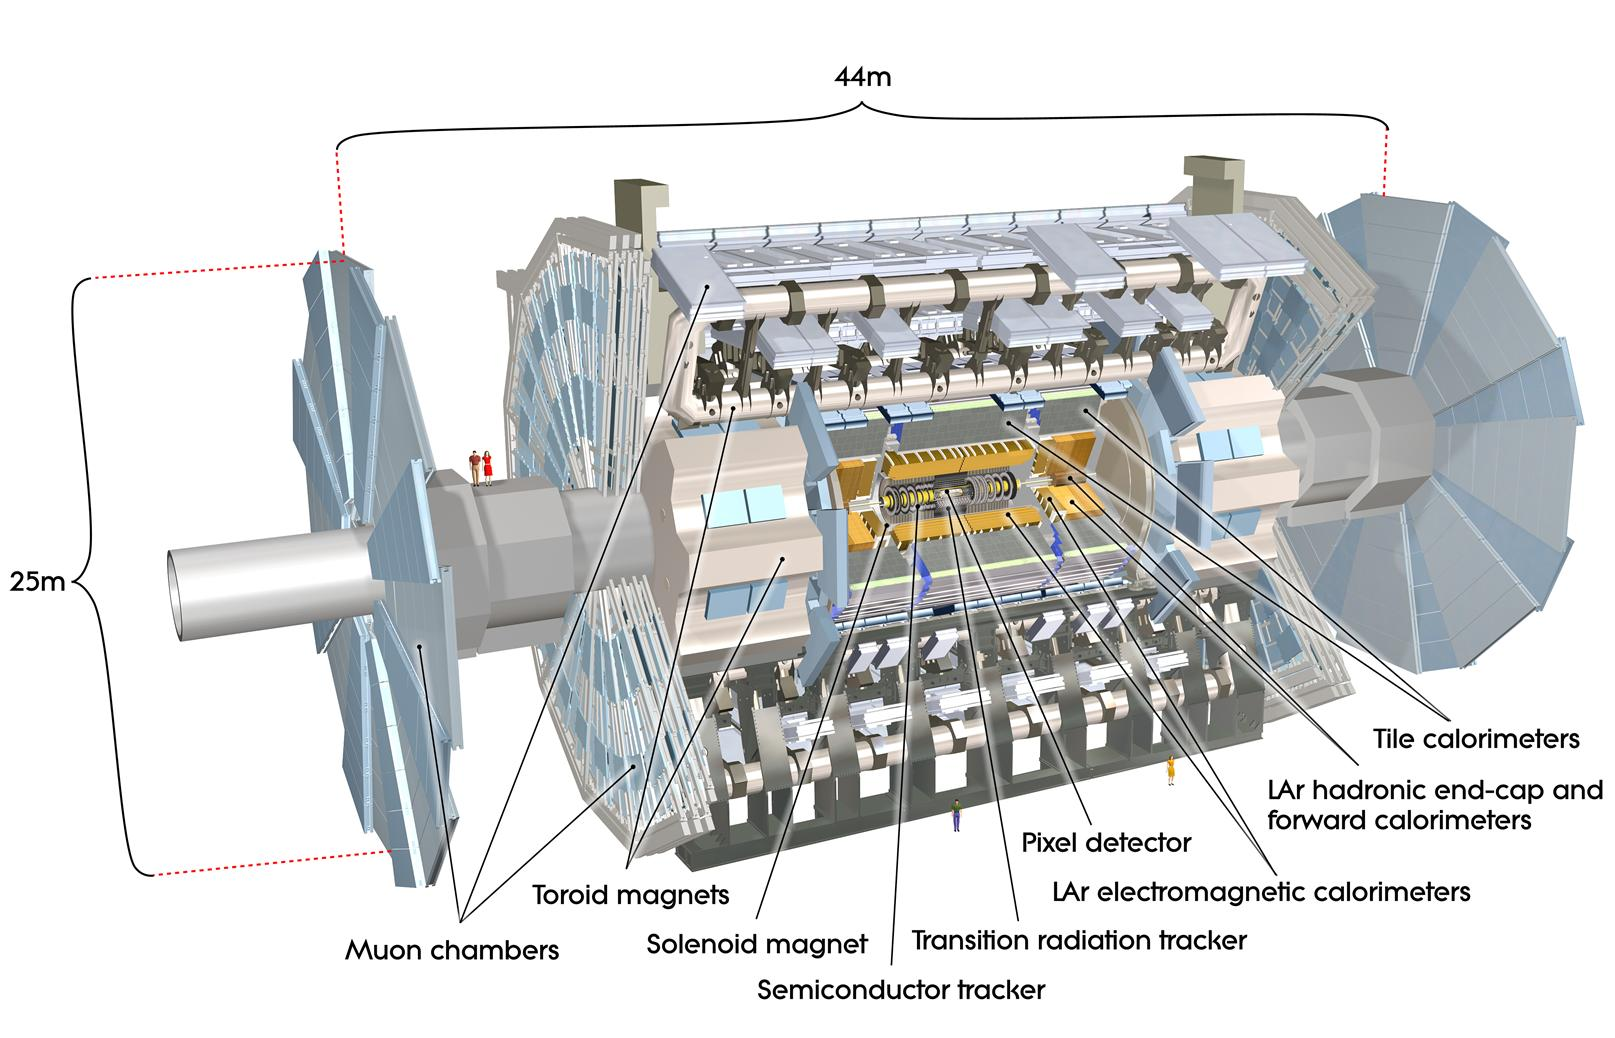
\includegraphics[width=0.8\textwidth]{chapters/c4/figures/atlas.jpg}
 \end{center}
 \caption{Cut-away view of the ATLAS detector}
 \label{fig:cutaway}
\end{figure}

\par The four major components of the ATLAS detector are the Inner Detector, the Calorimeter, the Muon Spectrometer, and the Magnet System. Integrated with the detector components are: the Trigger and Data Acquisition System, a specialized multi-level computing system, which selects physics events with distinguishing characteristics; and the Computing System, which develops and improves computing software used to store, process and analyze vast amounts of collision data at 130 computing centers worldwide\cite{atlas}.

\begin{figure}[htbp]
 \begin{center}
 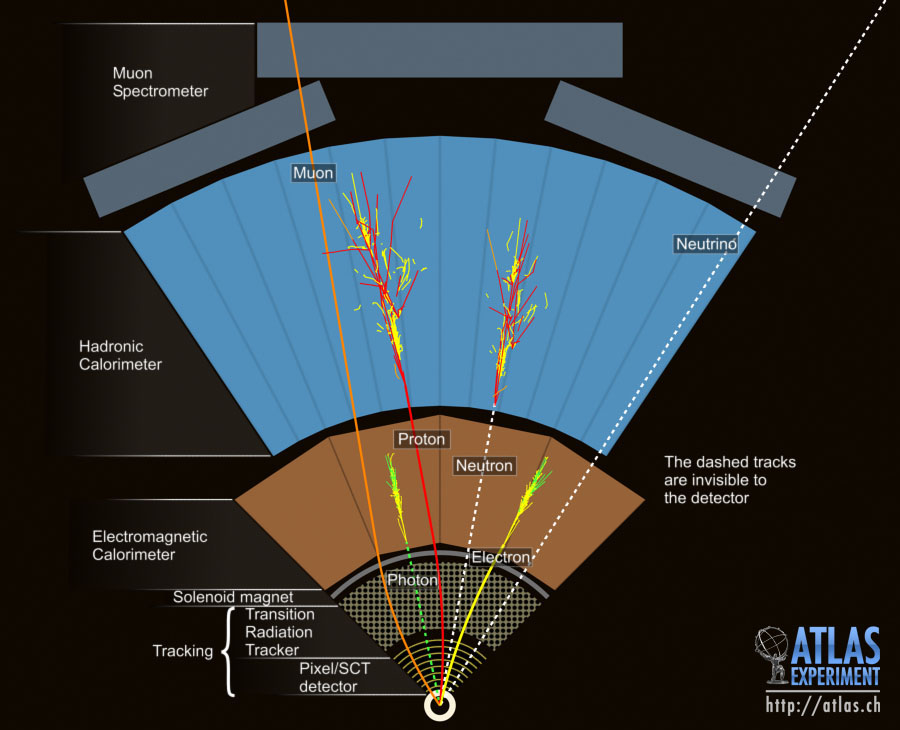
\includegraphics[width=0.8\textwidth]{chapters/c4/figures/eve_gen.jpg}
 \end{center}
 \caption{An image of
the ATLAS detector, showing the
different layers and the interactions
of different particle types through
the layers.}
 \label{fig:eve-gen}
\end{figure}

\par Different particles deposit energy in different layers as shown in Fig~\ref{fig:eve-gen}, where inner Detectors measure $\frac{q}{p_T}$ (charge over transverse momentum), the measurement of charged particles, Calorimeters measure energy of electromagnetically and hadronically interacting particles, and the Muon Spectrometer serves as an tracker for muons.

\par This chapter is intended as a brief introduction to the ATLAS sub-systems, including Inner Detectors in Section~\ref{sec:inner}, calorimeters in Section~\ref{sec:calo}, muon system in Section~\ref{sec:muon}, Forward detectors in Section~\ref{sec:for}, and trigger and data acquisition system in Section~\ref{sec:data}.

\section{Inner detector}
\label{sec:inner}
\begin{figure}[htbp]
 \begin{center}
 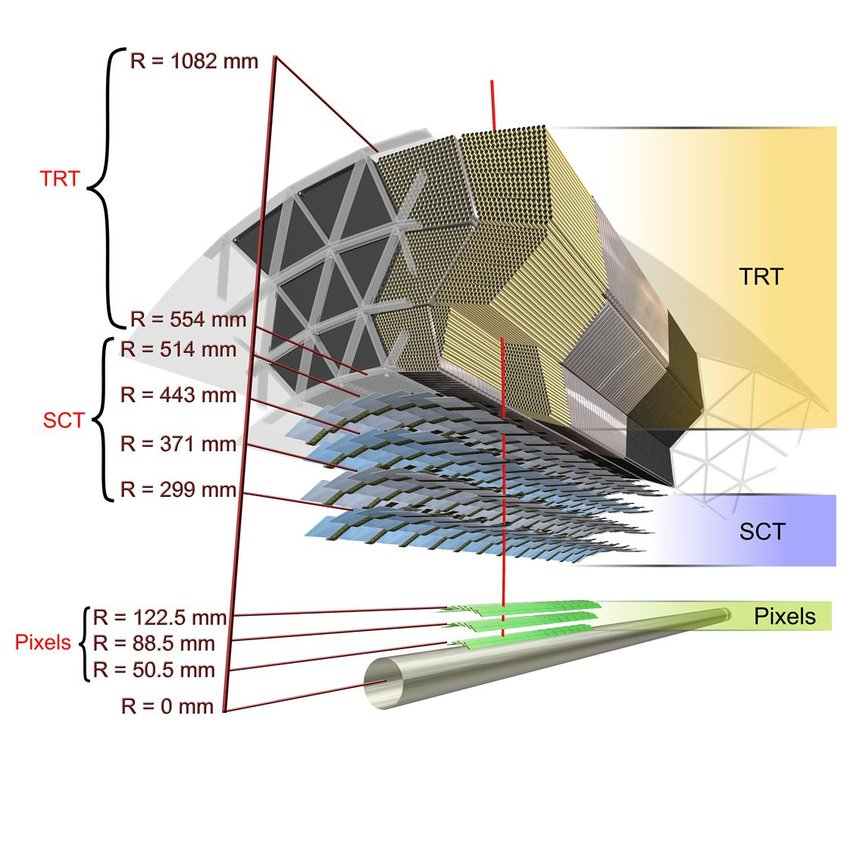
\includegraphics[width=0.8\textwidth]{chapters/c4/figures/inner}
 \end{center}
 \caption{Cut-away view of the ATLAS Inner Detector.}
 \label{fig:inner}
\end{figure}

\par The Inner Detector tracker is important for track reconstruction as well as both primary and secondary vertex measurements for charged tracks in the pseudorapidity range of $ \eta< 2.5$. The Inner Detector tracker is contained within a cylindrical envelope with a length of $\pm$3512 millimeter and a radius of 1150 millimeter.

\par As shown in Fig~\ref{fig:inner}, the Inner Detector tracker comprises three detector types dedicated to tracking. Moving from inside out we find the Silicon Pixel Detector, the SemiConductor Tracker (SCT), and the Transition Radiation Tracker (TRT). An extra pixel detector layer (IBL)\cite{Capeans:1291633} was inserted before the Run 2 and improves the identification of b-jets \cite{ATL-PHYS-PUB-2015-022}. The Pixel system provides a coverage of $|\eta|<2.5$. The SCT system consists of four barrel double layers and 18 end-cap layers (9 on each end) \cite{Aad:2014mta}, and provides a coverage of $|\eta| < 2.5$. The TRT consists of 70 barrel layers and 280 end-cap layers (140 on each end), and provides a coverage of $|\eta| < 2.0$\cite{Aad:2014mta}.

\subsection{Pixel detector}
\label{sec:pixel}

\begin{figure}[htbp!]
\begin{subfigure}{.5\textwidth}
 \centering
 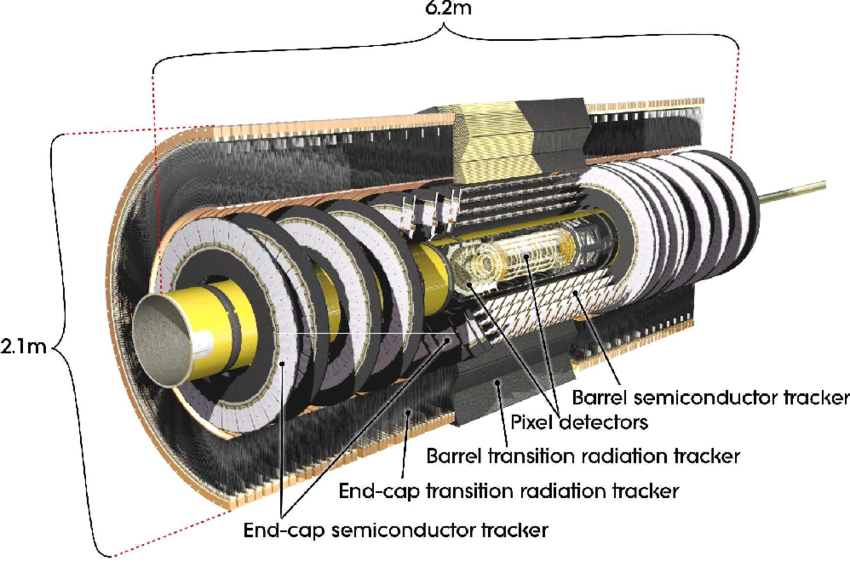
\includegraphics[width=0.8\textwidth]{chapters/c4/figures/pixel}
 \caption{a}
 \label{fig:pixel1}
\end{subfigure}%
\begin{subfigure}{.5\textwidth}
 \centering
 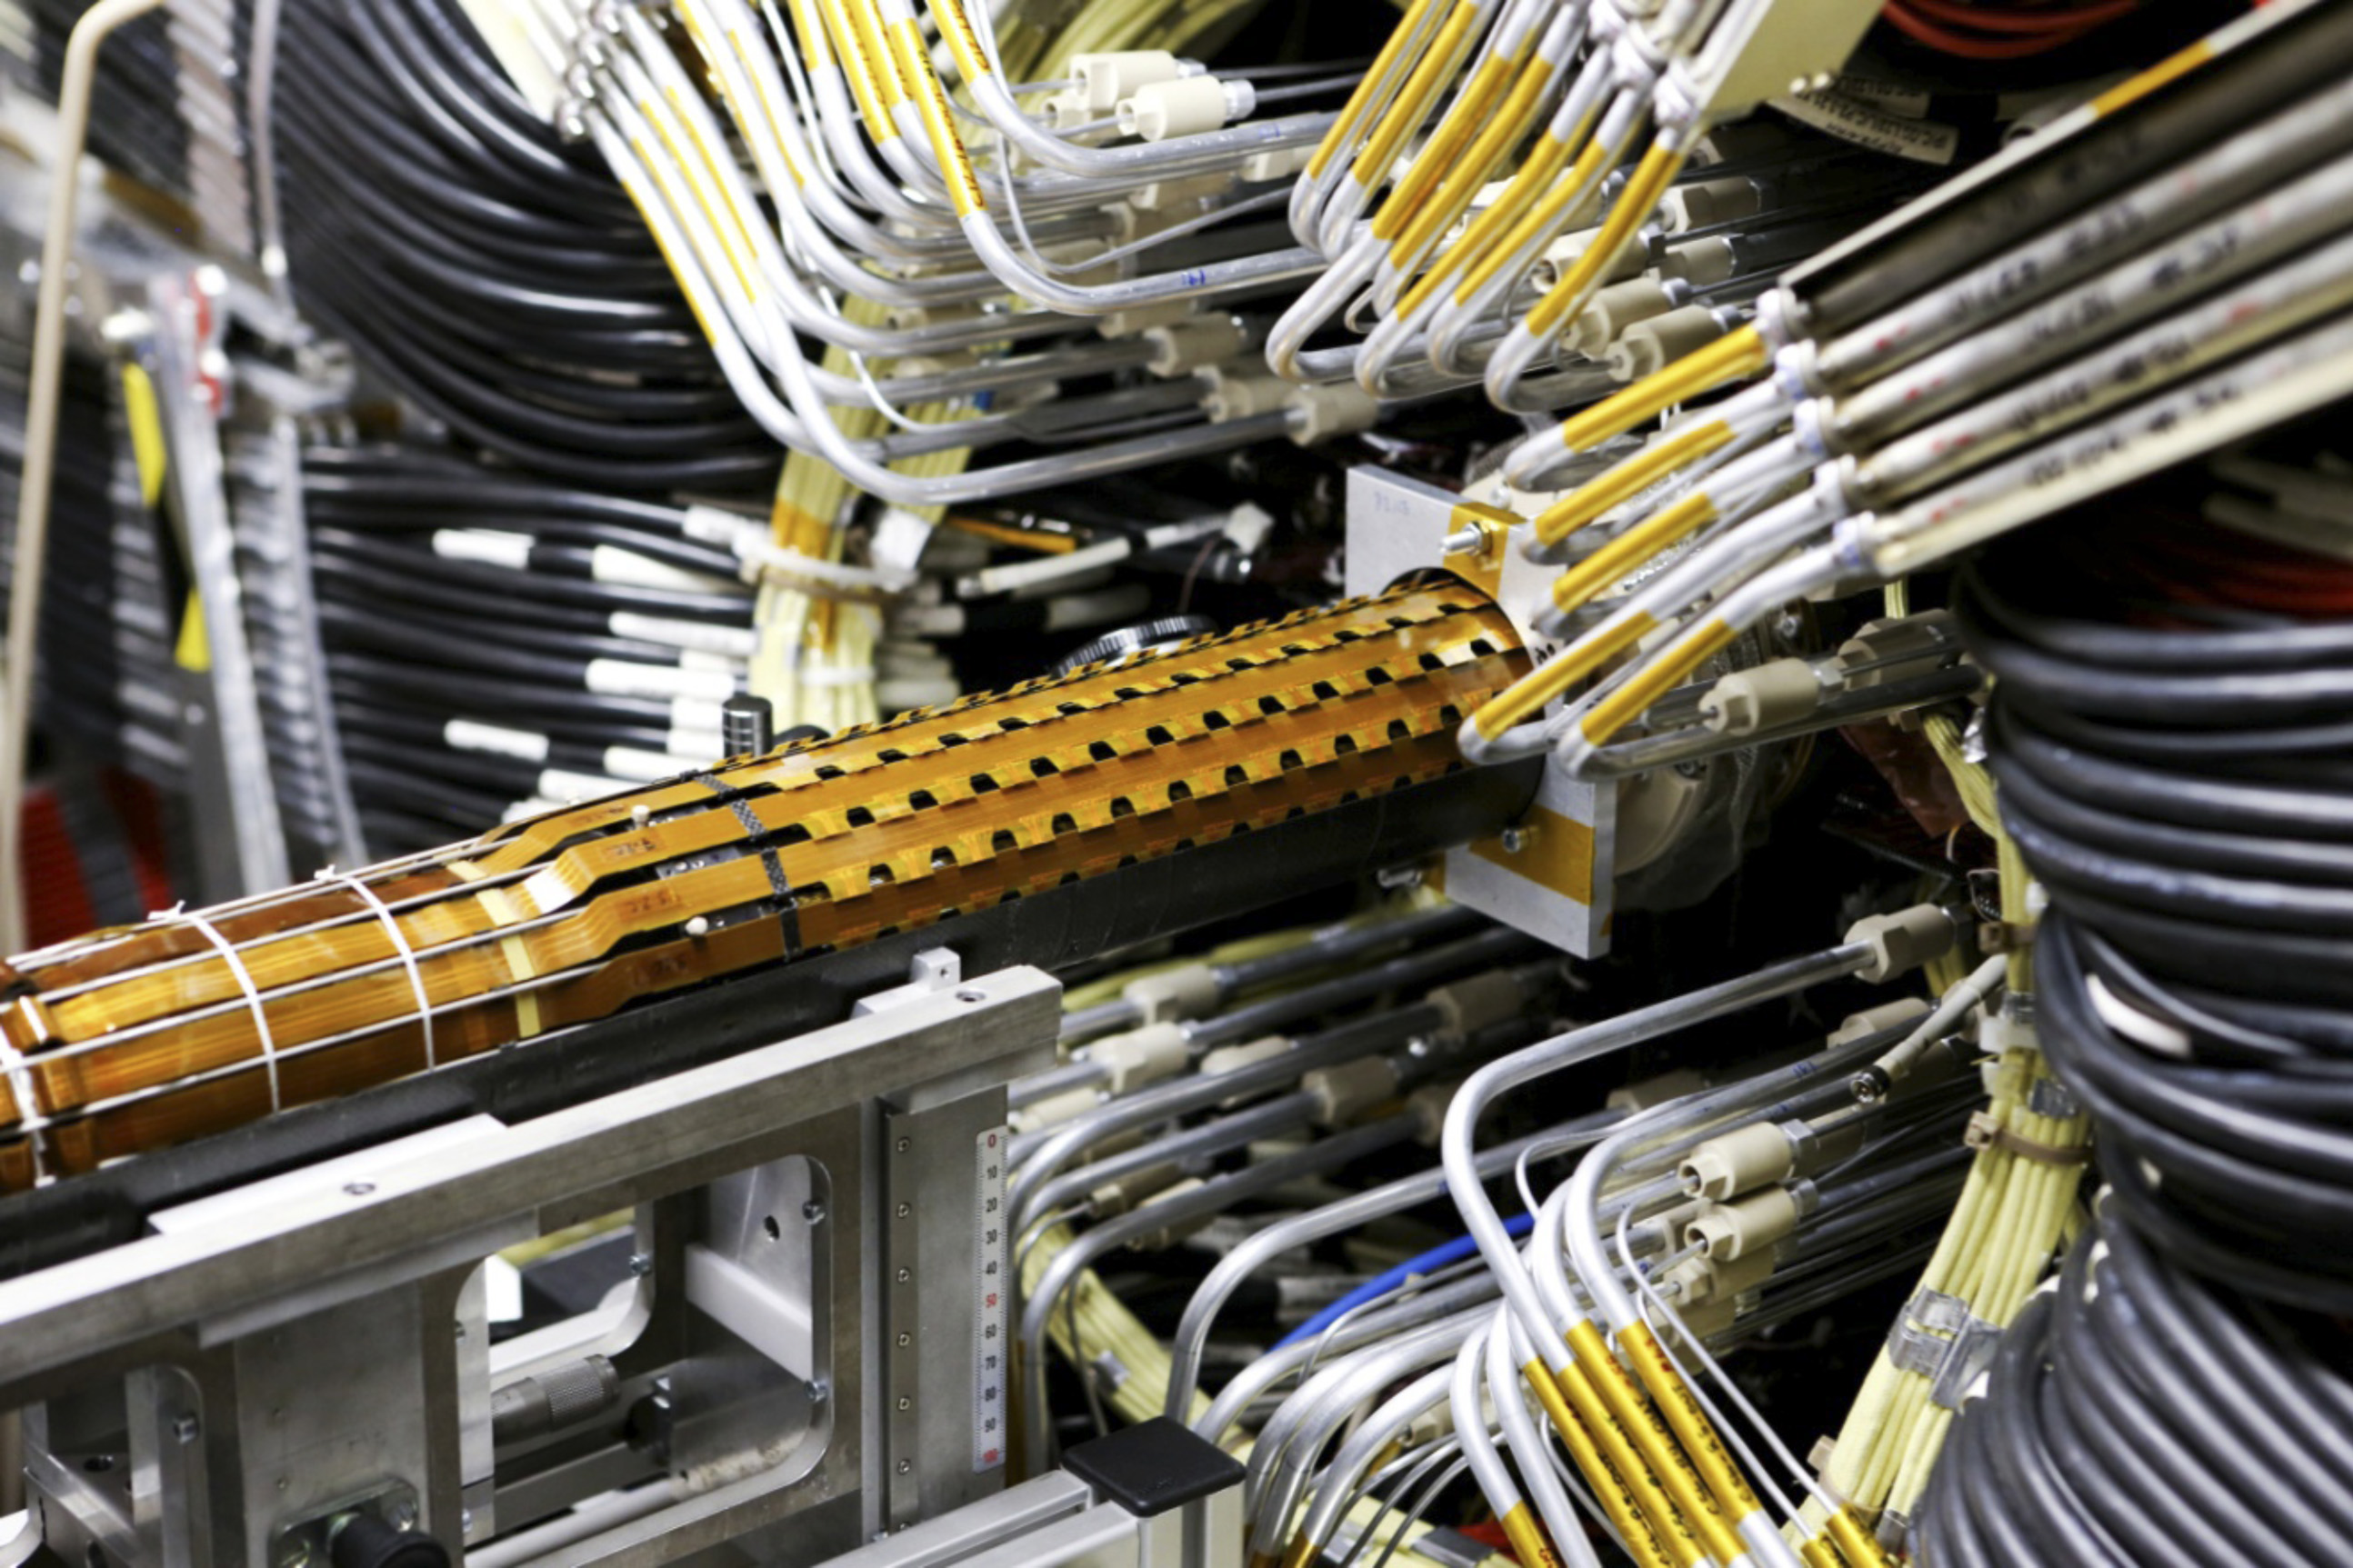
\includegraphics[width=0.8\textwidth]{chapters/c4/figures/IBL}
 \caption{b}
 \label{fig:pixel2}
\end{subfigure}
 \caption{A schematic view of the active region of the Pixel detector consisting of barrel and end-cap layers (\ref{fig:pixel1}) and the IBL detector before the insertion (\ref{fig:pixel2})}
\label{fig:pixel}
\end{figure}

\par The Pixel detector is the innermost element of the Inner Detector \cite{Hirono:2641635}. With the fine granularity of the pixel sensors, the pixel detector is designed to provide the identification and reconstruction of secondary vertices from the long-lived particles. It provides high resolution for primary vertices reconstruction to suppress pile-ups due to the increase of luminosity for LHC. A schematic view of the active region of the pixel detector consisting of a barrel and end-cap layers can be found in Fig~\ref{fig:pixel1}.

\par The IBL makes it possible for the pixel detector to have further improved resolution and a picture of the IBL being inserted into the Pixel detector is shown in Fig~\ref{fig:pixel2}. The pixel sensor pitch of the IBL has a minimum size in $R-\phi \times z$ of $50 \times 250~\mu m^2$ compared to other pixel detector layers with a size of $50 \times 400~\mu m^2$. The IBL provides an intrinsic spatial resolution for hits of $14~\mu m$ in the $R-\phi$ plane, and $72~\mu m$ in the z-direction, compared to an intrinsic spatial resolution for hits of $14\mu m$ in the $R-\phi$ plane, and $115~\mu m$ in the z-direction of the three outer pixel barrel layers.

\par The Pixel detector's ability to associate tracks correctly to secondary vertices is essential to tagging algorithms of the $b$-hadrons decays which are important for this thesis, as well as other non-prompt decays.

\subsection{Semiconductor Tracker~(SCT)}
\par The SCT \cite{AHMAD200798} is designed to provide a good measurement of momentum, impact parameter, and vertexes. It includes 4 cylindrical barrel layers and 18 planar end-cap disks, covered by $61 m^2$ of silicon detectors and 6.2 million readout channels. The spatial resolution is about $16~\mu m$ in the $R-\phi$ plane and $580~\mu m$ in the z-direction.

\subsection{Transition Radiation Tracker~(TRT)}
\par The TRT\cite{Abat:2008zza} is the outermost part of the Inner Detector. The TRT is composed of thin proportional chambers either in the form of straws embedded in fibers or with foils. The 4-mm diameter Kapton straw drift tubes, which can be operated at 6 to 18 MHz at the barrel while 7 to 19 MHz at the end-caps, are filled with a mixture gas. The mixture gas is composed with 70\% of Xe, 20\% of $CF_{4}$ and 10\% of $CO_{2}$.

\par The TRT is designed as a dual-purpose detector: quasi-continuous tracking and particle identification. The quasi-continuous track reconstruction is achieved by the large amount of hits provided by 370000 straws in TRT. The particle is identified by its transition radiation product when it is traveling across the material boundaries ($CO_{2}$ gas and polypropene/polyethene fibers). 

\section{Calorimeter}
\label{sec:calo}
\begin{figure}[htbp]
 \begin{center}
 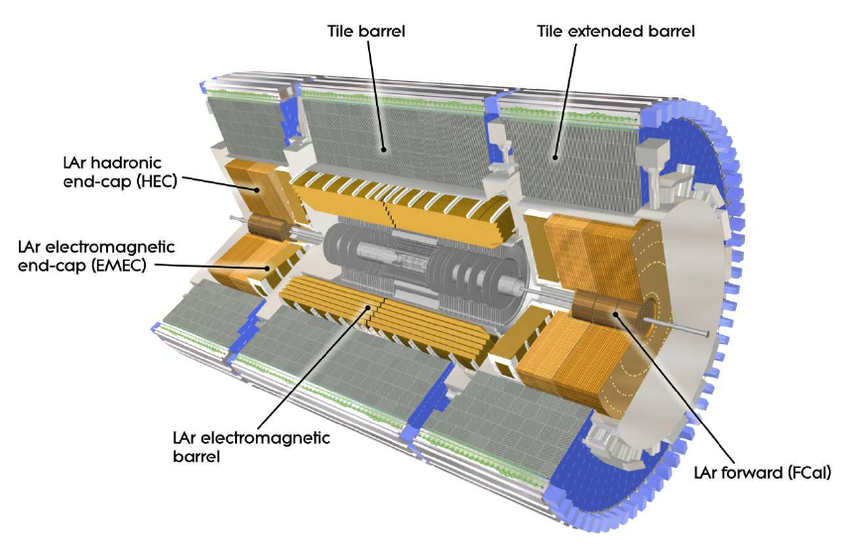
\includegraphics[width=0.8\textwidth]{chapters/c4/figures/Calo}
 \end{center}
 \caption{Cut-away view of ATLAS calorimeter system}
 \label{fig:Calo}
\end{figure}

\par The ATLAS calorimeters \cite{CERN-LHCC-96-041} are designed to measure the energy of the outgoing particles. Particles passing the calorimeters will initiate particle showers, either electromagnetic (EM) showers (consisting of electrons and photons) or hadronic showers (consisting of pions , protons, ...) in layers of passive material made of dense materials. Such showers grow as the outgoing particles continue to interact with the absorber until their energies are lower than the critical energy where the ionization becomes dominant over radiation or interactions. The ATLAS calorimeters are sampling calorimeters with layers where the final state particles can induce ionization or scintillation in the active layers to record the energy of the showering particles.

\par There are two types of calorimeters in ATLAS as shown in Fig~\ref{fig:Calo}: the EM calorimeter, a lead/liquid-argon sampling calorimeter, covering the pseudorapidity range of $|\eta| < 1.475$ in the barrel region and $1.375 < |\eta| < 3.2$ in the end-cap region; the hadronic calorimeter, consisting of the tile calorimeter covering $|\eta| < 1.7$, the liquid-argon hadronic end-cap calorimeter (HEC) covering $1.5 < |\eta| < 3.2$; and the liquid-argon forward calorimeter (FCal) covering $3.1 < |\eta| < 4.9$.

\par To contain all particles showers in the calorimeters and thus avoiding particles (except muons and neutrinos) penetrating into the muon spectrometer, the materials and thickness of each layers are optimized \cite{Aad:1129811}. The thickness of the EM calorimeter is greater than 22 $X_0$ in the barrel and 24 $X_0$ in the end-cap region, where the radiation length of the material $X_0$ represents the thickness of material that reduces the mean energy of an electron by a factor $e$. The thickness of the hadronic calorimeter is approximately 9.7$~\lambda$ in the barrel and 10$~\lambda$ in the end-cap regions, where $\lambda$ is the nuclear interaction length.

\par Ideally, if all showers are counted, the measured energy would be proportional to the signal strength and thus the error is proportional to $\sqrt{E}$:

\begin{equation}
\label{eq:timeresn}
\frac{\sigma(E)}{E} = \frac{a}{\sqrt{E}} \oplus \frac{b}{E} \oplus c \ \ \  ,
\end{equation}
where a is stochastic term, which is a combination of the intrinsic statistical shower fluctuation, signal quantum fluctuation and sampling fluctuation, b is a noise term from readout electronics noise, radioactivity and pile-up fluctuations, and c is a constant term representing any inhomogeneities and imperfections in calorimeter construction, and non-linearity of readout electronics \cite{calorimetry}. From Equation~\ref{eq:timeresn}, we could the energy resolution improves with increasing energy in general.

\subsection{Liquid Argon Calorimeter}

\par The LAr EM Calorimeter uses lead as its passive material, and the active material is liquid argon (LAr). 
It consists of the barrel EM calorimeter (EMB) and one end-cap (EMEC) on each side, with the inner wheels (IW) covering 1.375 $< |\eta| <$ 2.5 and outer wheels (OW) covering 2.5 $< |\eta| <$ 3.2.

\begin{figure}[htbp!]
\begin{subfigure}{.5\textwidth}
 \centering
 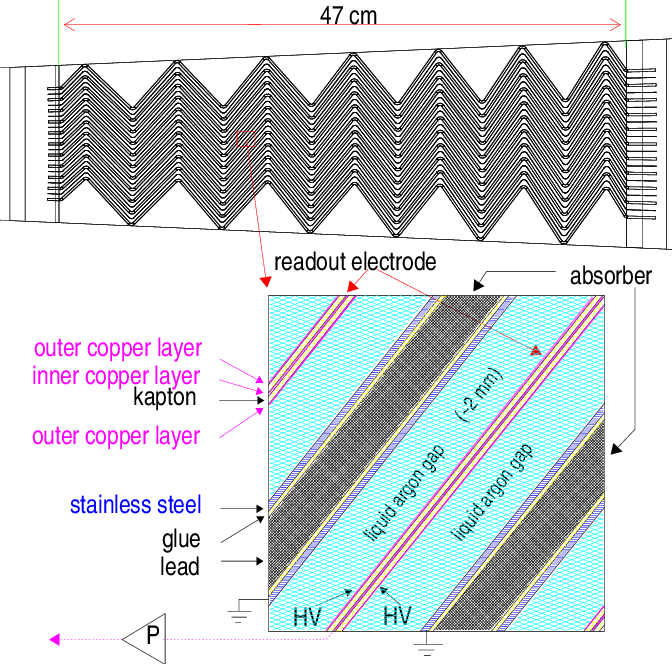
\includegraphics[width=0.8\textwidth]{chapters/c4/figures/lar-layers}
 \caption{a}
 \label{fig:lar1}
\end{subfigure}%
\begin{subfigure}{.5\textwidth}
 \centering
 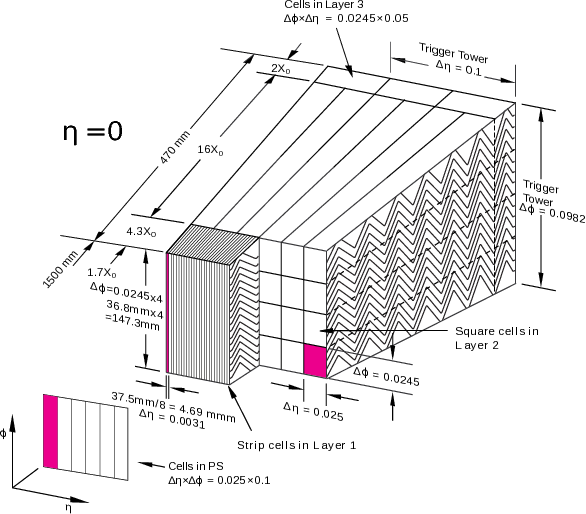
\includegraphics[width=0.8\textwidth]{chapters/c4/figures/lar}
 \caption{b}
 \label{fig:lar2}
\end{subfigure}
 \caption{Accordion structure of the barrel. The left figure is a view of a small sector of the barrel calorimeter in a plane transverse to the LHC beams. The right figure is a diagram of a sketch of barrel module showing both accordion structure and granularity in $\eta - \phi$ of the cells on each of layer}
 \label{fig:pixel}
\end{figure}

\par As shown in Fig~\ref{fig:lar1}, the LAr calorimeter uses a novel accordion geometry to avoid gaps at boundaries. It comprises accordion-shaped copper-kapton electrodes positioned between lead absorber plates and kept in position by honeycomb spacers while the system is immersed in LAr. The accordion geometry provides complete $\phi$ coverage without azimuthal cracks.

\par For most of the EM calorimeter, EMB and EMEC-OW, each module has three layers in depth with different granularities, 
as can be seen in Fig~\ref{fig:lar2}, while each EMEC-IW module has only two layers. Table 1.3 of Ref~\cite{Aad:1129811} 
shows the granularity of the EM calorimeter for different ranges. The fine segmentation of the first layers helps distinguishing photons from $\pi_0$ mesons decaying to two photons, as well as providing flight direction of neutral particles. The second layers has a relatively coarser granularity but it is quite thick so the largest fraction of the energy is deposited there, and only a small tail of the EM shower penetrates in the last layer which measures the remaining energy of the most energetic particles.

\par The principle of operation of the HEC and FCal is similar to LAr, but they use copper and tungsten as passive material and the design details are different and vary with position.

\subsection{Tile Calorimeter}

\par Located outside of the LAr EM calorimeter, the tile calorimeter~\cite{CERN-LHCC-96-042} is a sampling calorimeter using steel as the absorber and scintillator as the active medium. Its barrel covers the region $|\eta| <$ 1.0, and its two extended barrels covers the range 0.8 $< |\eta| <$ 1.7.

\par The barrel and extended barrels are divided azimuthally into 64 modules with a span $\Delta \phi = 0.1$. It is segmented in depth in three layers, approximately 1.5 $\lambda$, 4.1 $\lambda$ and 1.8 $\lambda$ thick for the barrel and 1.5 $\lambda$, 2.6 $\lambda$, and 3.3 $\lambda$ for the extended barrel.

\begin{figure}[htbp!]
 \begin{center}
 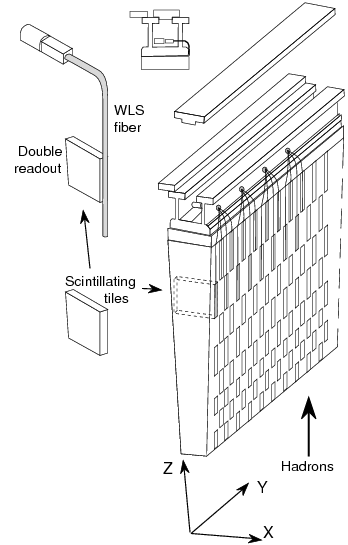
\includegraphics[width=0.6\textwidth]{chapters/c4/figures/tile}
 \end{center}
 \caption{Illustration of a Tile calorimeter module.}
 \label{fig:Tile}
\end{figure}

\par As shown in Fig~\ref{fig:Tile}, scintillator tiles are oriented radially, with wavelength-shifting readout fiber connected at the tile edge. Readout fibers are then grouped together and are connected to the readout photomultiplier.

\section{Muon Spectrometer (MS)}
\label{sec:muon}

\begin{figure}[htbp!]
\begin{subfigure}{.5\textwidth}
 \centering
 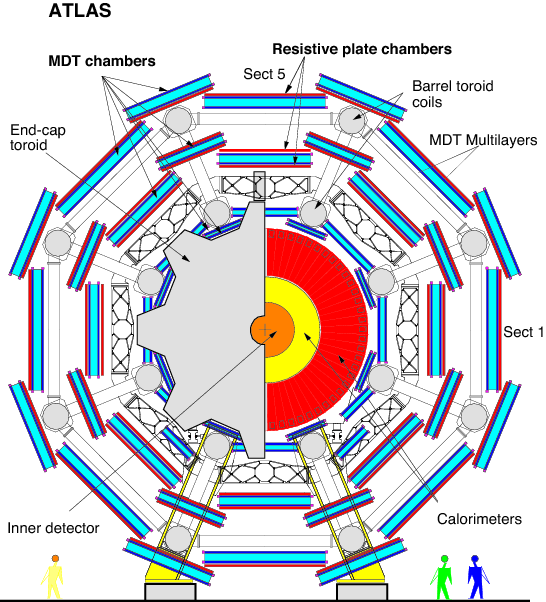
\includegraphics[width=0.8\textwidth]{chapters/c4/figures/mu-bar}
 \caption{a }
 \label{fig:mu-bar}
\end{subfigure}%
\begin{subfigure}{.5\textwidth}
 \centering
 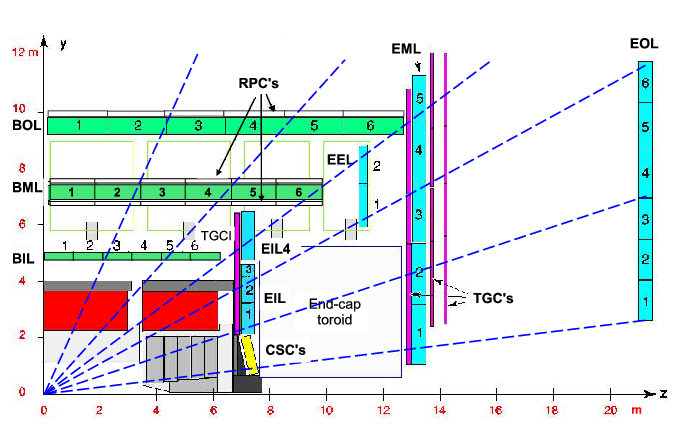
\includegraphics[width=0.8\textwidth]{chapters/c4/figures/mu-end}
 \caption{b}
 \label{fig:mu-end}
\end{subfigure}
 \caption{Geometric layout of muon sub-detectors in barrel (\ref{fig:mu-bar}) and end-cap (\ref{fig:mu-end}) region}
\label{fig:mu}
\end{figure}

\par The MS \cite{CERN-LHCC-97-022} is designed to measure the trajectory of transversing muons, as well as to provide muon trigger signals using separate sets of detection chambers. The MS is immersed in a toroidal magnetic field of about 0.5 T and 1 T in the barrel and end-cap regions, respectively. The MS is designed to measure muons standalone in a wide range of 3 GeV up to about 3 TeV. Being located farthest from interaction point, cells are relatively large due to low occupancy and the radiation level is typically smaller in the muon system. Also, it should be able to perform standalone measurement of high-momentum muon \cite{muon}.
The targeted $p_T$ resolution is 10\% for 1 TeV muon tracks, which is a sagitta along the z-axis of about 500 $\mu m$ with a resolution of about 50 $\mu m$.

\par As illustrated in Fig~\ref{fig:mu}, the MS is composed of the precision tracking detectors, Monitored Drift-tube Chambers (MDT) and Cathode Strip Chambers (CSC), as well as the triggering detectors, Resistive Plate Chambers (RPC) in the barrel region and Thin Gap Chambers (TGC) in the end-cap region.

\par MDTs have a spatial resolution of about 80 $\mu m$ and cover $|\eta| < 2.7$, except in the innermost end-cap layer, where it is $|\eta| < 2.0$. The CSCs with higher rate capability are installed on the forward region of $2.0 < |\eta| < 2.7$ in the innermost end-cap layer. They have a resolution of about 60$\mu m$, but since the cathode segmentation is coarser, the resolution is 5 mm in the non-bending direction. RPCs in the barrel region covering $|\eta| < 1.05$ and TGCs in the end-cap region covering $1.05 < |\eta| < 2.4$ provide a very fast response to muon hits.

\par Muon reconstruction and identification algorithms rely on information from both the Inner Detector and the MS.

\section{Forward Detectors}
\label{sec:for}
\begin{figure}[htbp]
 \begin{center}
 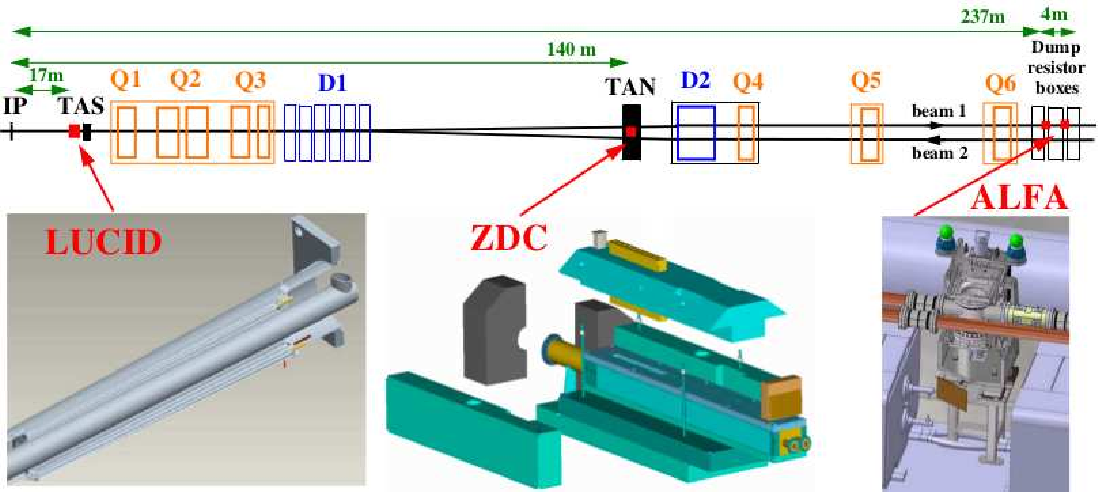
\includegraphics[width=0.8\textwidth]{chapters/c4/figures/forward}
 \end{center}
 \caption{Cut-away view of the ATLAS Inner Detector.}
 \label{fig:forward}
\end{figure}

\par Shown in Fig~\ref{fig:forward}, LUCID (Luminosity measurement using Cerenkov Integrating Detector), ALFA (Absolute Luminosity For ATLAS) and ZDC (Zero-Degree Calorimeter) are together called Forward Detectors. 

\par The LUCID and ALFA are dedicated to luminosity measurement at ATLAS experiment. The LUCID, situated at 17 meter from the interaction point on both side, is a luminosity monitor that able to monitor online bunch-by-bunch luminosity and provide absolute luminosity after calibration. The ALFA, housed in Roman pots at 240m, is designed to measure the total cross section. It will provide simultaneously total cross section and luminosity with an uncertainty of 2-3\% in the LHC working range. The ZDC, located at 140 meter from the interaction point, although it is designed to study heavy ions and proton-proton physics, it can also be used as luminosity monitor to tune the LHC parameters during the first day machine adjustment (for example, Van der Meer scan).

\section{Trigger and Data Acquisition}
\label{sec:data}

\begin{figure}[htbp!]
 \centering
 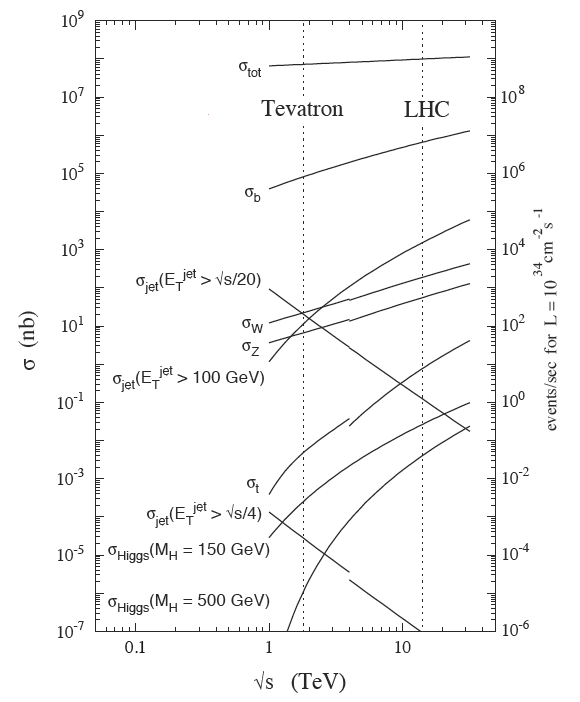
\includegraphics[width=0.8\textwidth]{chapters/c4/figures/cross}
 \caption{b}
 \label{fig:cross}
 \caption{Cross sections of physics processes produced by hadron colliders~\ref{fig:cross}}
\end{figure}

\par As illustrated in Fig~\ref{fig:lumi}, the cumulative luminosity delivered by LHC during Run 2 is about 156~fb$^{-1}$. However, as shown in Fig~\ref{fig:cross}, the rate of events containing electroweak bosons, top quarks or high \pt jets physics phenomena is a tiny fraction of total events. So the trigger system is a key component of hadron collider experiments. In order to select events for a limited data storage capacity, the trigger system needs to provide fast online selection of events from a variety of physics processes to record for later analysis.

\begin{figure}[htbp!]
 \begin{center}
 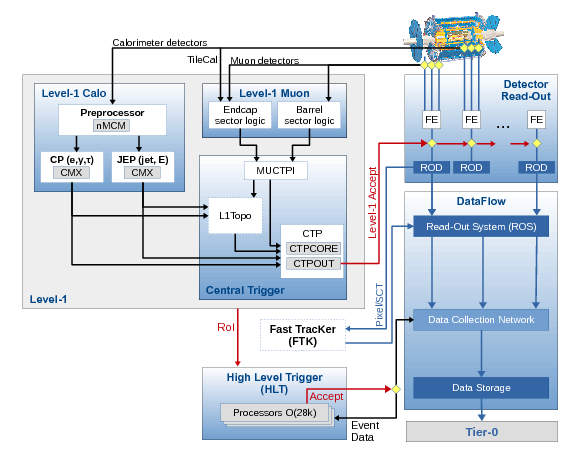
\includegraphics[width=0.8\textwidth]{chapters/c4/figures/TDAQ}
 \end{center}
 \caption{The ATLAS TDAQ system in Run 2 with the relevant components for triggering. }
 \label{fig:TDAQ}
\end{figure}

\par The ATLAS Trigger and Data Acquisition (TDAQ) system \cite{Ruiz-Martinez:2133909} is illustrated in Fig~\ref{fig:TDAQ}. In Run 2, the trigger system consists of two levels of event selections: the Level 1 trigger (L1) is a hardware-based trigger using reduced-granularity information from subdetectors, the ATLAS calorimeter (L1Calo) and Muon Spectrometer (L1 muon trigger). These send trigger information to the L1 Central Trigger Processor (CTP) which generates a pre-scale and final L1 decision (L1A) signal. The front-end of each sub-detector receives the L1A and transmits the data for selected events off-detector. The rate of L1As is about 100 kHz, reducing the total 40 MHz event rate by a factor of 400. This is followed by a software-based High Level Trigger (HLT) that reduces the rate to 1 kHz on average. Accepted events are reconstructed and sent to long-term storage. As a result, the L1 and HLT triggers together reduce the accepted event rate by a factor of 40000.
